\section{Simulation Analysis}
\label{sec:simulation}

Since this circuit is a steady one, the voltage or current values of the various components doesn't vary in time. Therefore, only the Operating Point Analysis is necessary in this circuit simulation

\subsection{Operating Point Analysis}


For this circuit's simulation on Ngspice, there was a need to introduce a null voltage source between the ground node and the R7 resistor. The voltage related to node V2 will not appear in following table~\ref{tab:op} because it has the same voltage as node V1 (its omission is necessary for the simulation to run correctly).

Table~\ref{tab:op} below shows the simulated operating point results for the circuit
under analysis.

Using the results of the theoretical analysis for mere guidance, we know the voltage values for the nodes: that should follow from our simulation. We know then in which direction the voltage drops happen and we use this order for all branches except the current sources. In the current sources the order follows the current flow of such sources, as it is norm in Ngspice. Following the order we stated for the other branches means that the current that flows through every resistor must have a positive value in table~\ref{tab:op}, because in resistors the voltage drop and current flow have the same direction (resistors always consume energy).

Analysing table~\ref{tab:op}, we notice that the current flowing through every resistor has a positive value, as it should be. I\textsubscript{a} is the current flowing through R1, I\textsubscript{b} is the current flowing through R2, I\textsubscript{c} is the current flowing through R6 (and R7), and, finally, I\textsubscript{d} is equivalent to Idd.
Comparing the simulation results for the voltage and current values with the theoretical analysis values, we notice that the values for voltage in nodes V\textsubscript{1} to V\textsubscript{9} and the current for all four mesh currents are exactly equal, if we exclude all roundings carried out by NgSpice, since its precision (up to 7 significant figures) can be slightly different than the precision we used in GNU Octave (a maximum of 2 significant figures of difference). Different digits only start to appear by the 6\textsuperscript{th} decimal case, which is a disposable calculation error (Shrinking the theoretical results to Ngspice precision, we get equal theoretical and simulation results).

With that being said, the theoretical results are equal to the simulation results (the complete accuracy is fruit of the staticness of the circuit), which confirms our theoretical analysis. The fact that the voltage and current results are equal obviously results in equal power values for each branch.

\begin{table}[h]
  \centering
  \begin{tabular}{|l|r|}
    \hline    
    {\bf Name} & {\bf Value [A or V]} \\ \hline
    @gb[i] & -2.29771e-04\\ \hline
@idd[current] & 1.005042e-03\\ \hline
@r1[i] & 2.191669e-04\\ \hline
@r2[i] & 2.297712e-04\\ \hline
@r3[i] & 1.060424e-05\\ \hline
@r4[i] & 1.185502e-03\\ \hline
@r5[i] & 1.234813e-03\\ \hline
@r6[i] & 9.663347e-04\\ \hline
@r7[i] & 9.663347e-04\\ \hline
v(1) & -9.73914e-01\\ \hline
v(3) & 1.063433e+01\\ \hline
v(4) & 6.382611e+00\\ \hline
v(5) & 6.843347e+00\\ \hline
v(6) & 7.067298e+00\\ \hline
v(7) & 1.953900e+00\\ \hline
v(8) & 6.875344e+00\\ \hline
v(9) & 0.000000e+00\\ \hline

  \end{tabular}
  \caption{Operating point analysis. A variable preceded by @ is of type {\em current}
    and expressed in Ampere; other variables are of type {\it voltage} and expressed in
    Volt.}
  \label{tab:op}
\end{table}

\begin{table}[h]
  \centering
  \begin{tabular}{|l|r|}
    \hline    
    {\bf Name} & {\bf Value [A or V]} \\ \hline
    \input{op2_tab}
  \end{tabular}
  \caption{Operating point analysis. A variable preceded by @ is of type {\em current}
    and expressed in Ampere; other variables are of type {\it voltage} and expressed in
    Volt.}
  \label{tab:op2}
\end{table}

\begin{figure}[h] \centering
\includegraphics[width=0.7\linewidth]{natura.pdf}
\caption{Simulated natural response for $V_{6}$ node voltage.}
\label{fig:natura}
\end{figure}

\begin{figure}[h] \centering
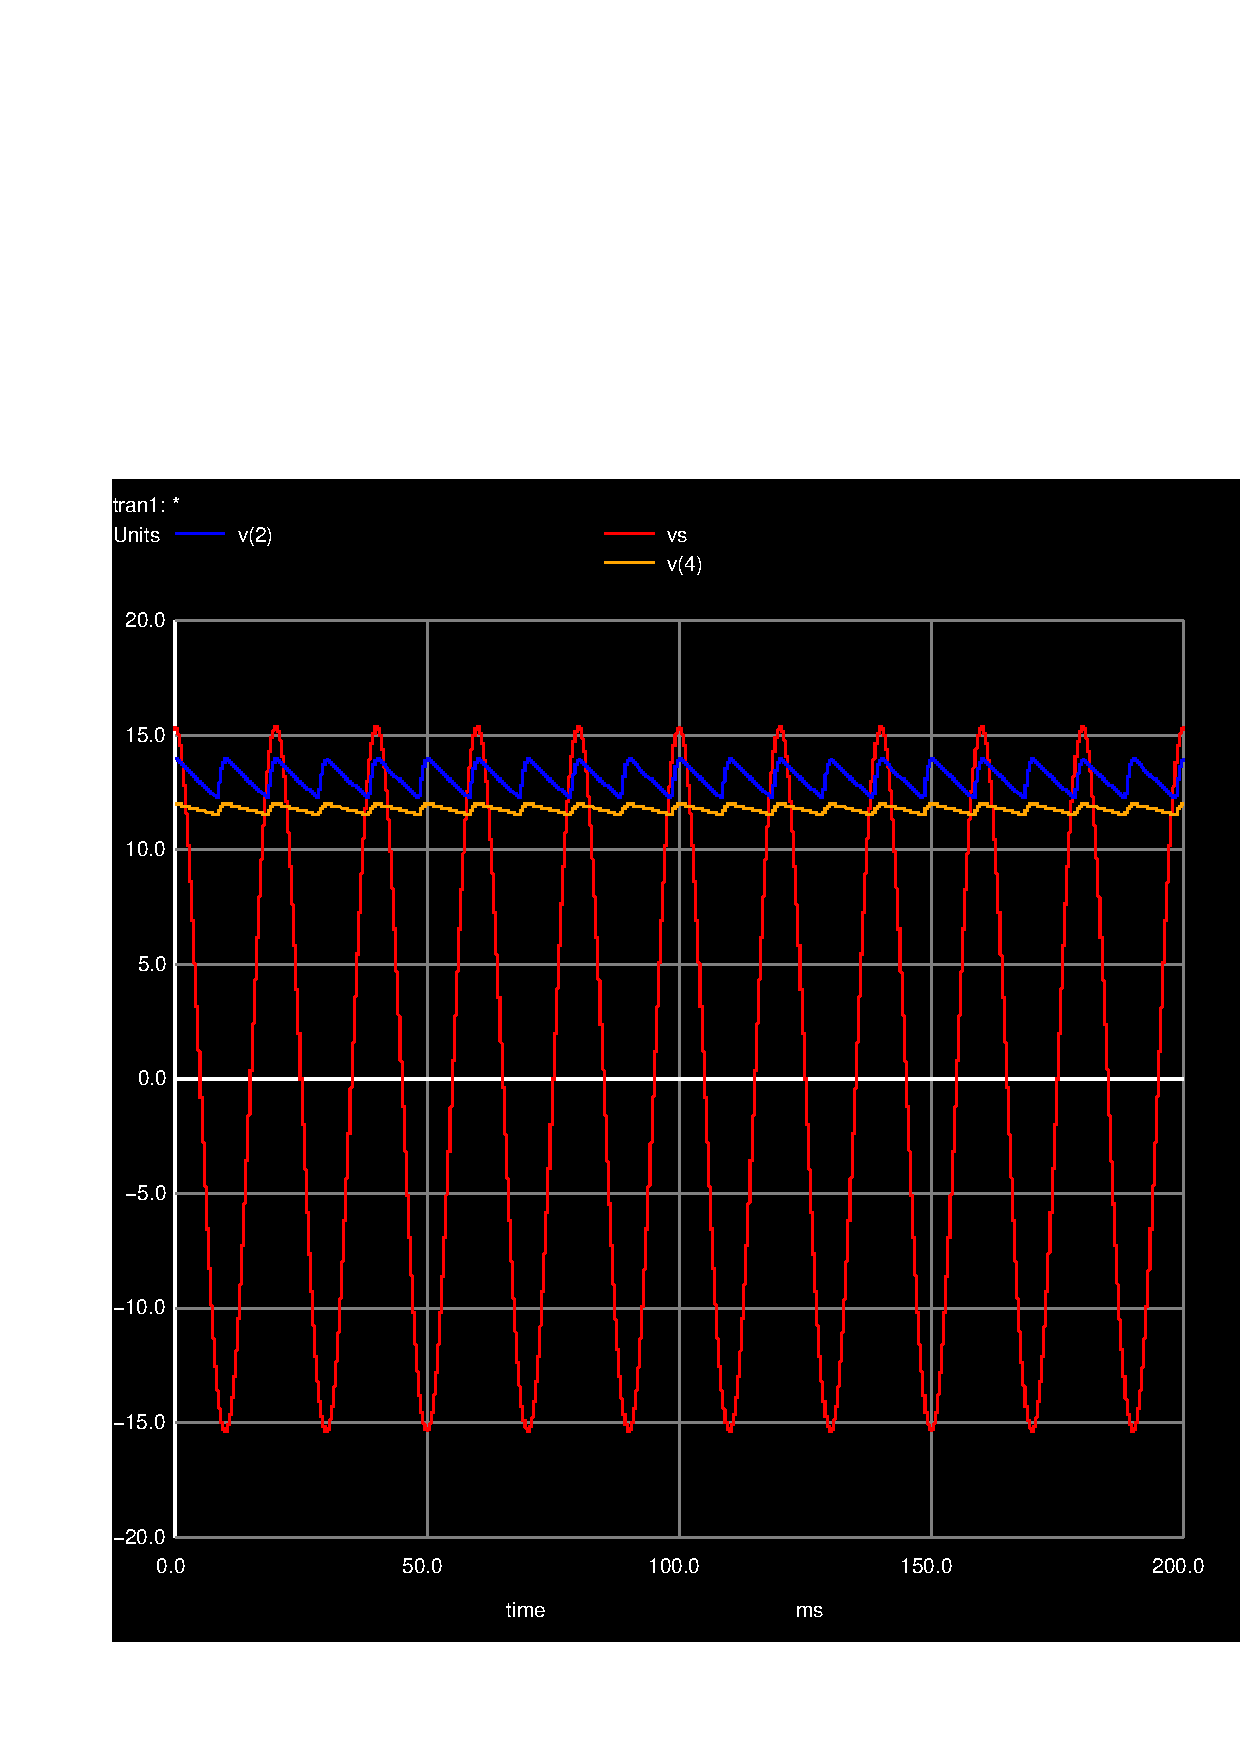
\includegraphics[width=0.7\linewidth]{total.pdf}
\caption{Simulated response for $V_{6}$ node voltage and stimulated voltage $V_{S}$.}
\label{fig:total}
\end{figure}

\begin{figure}[h] \centering
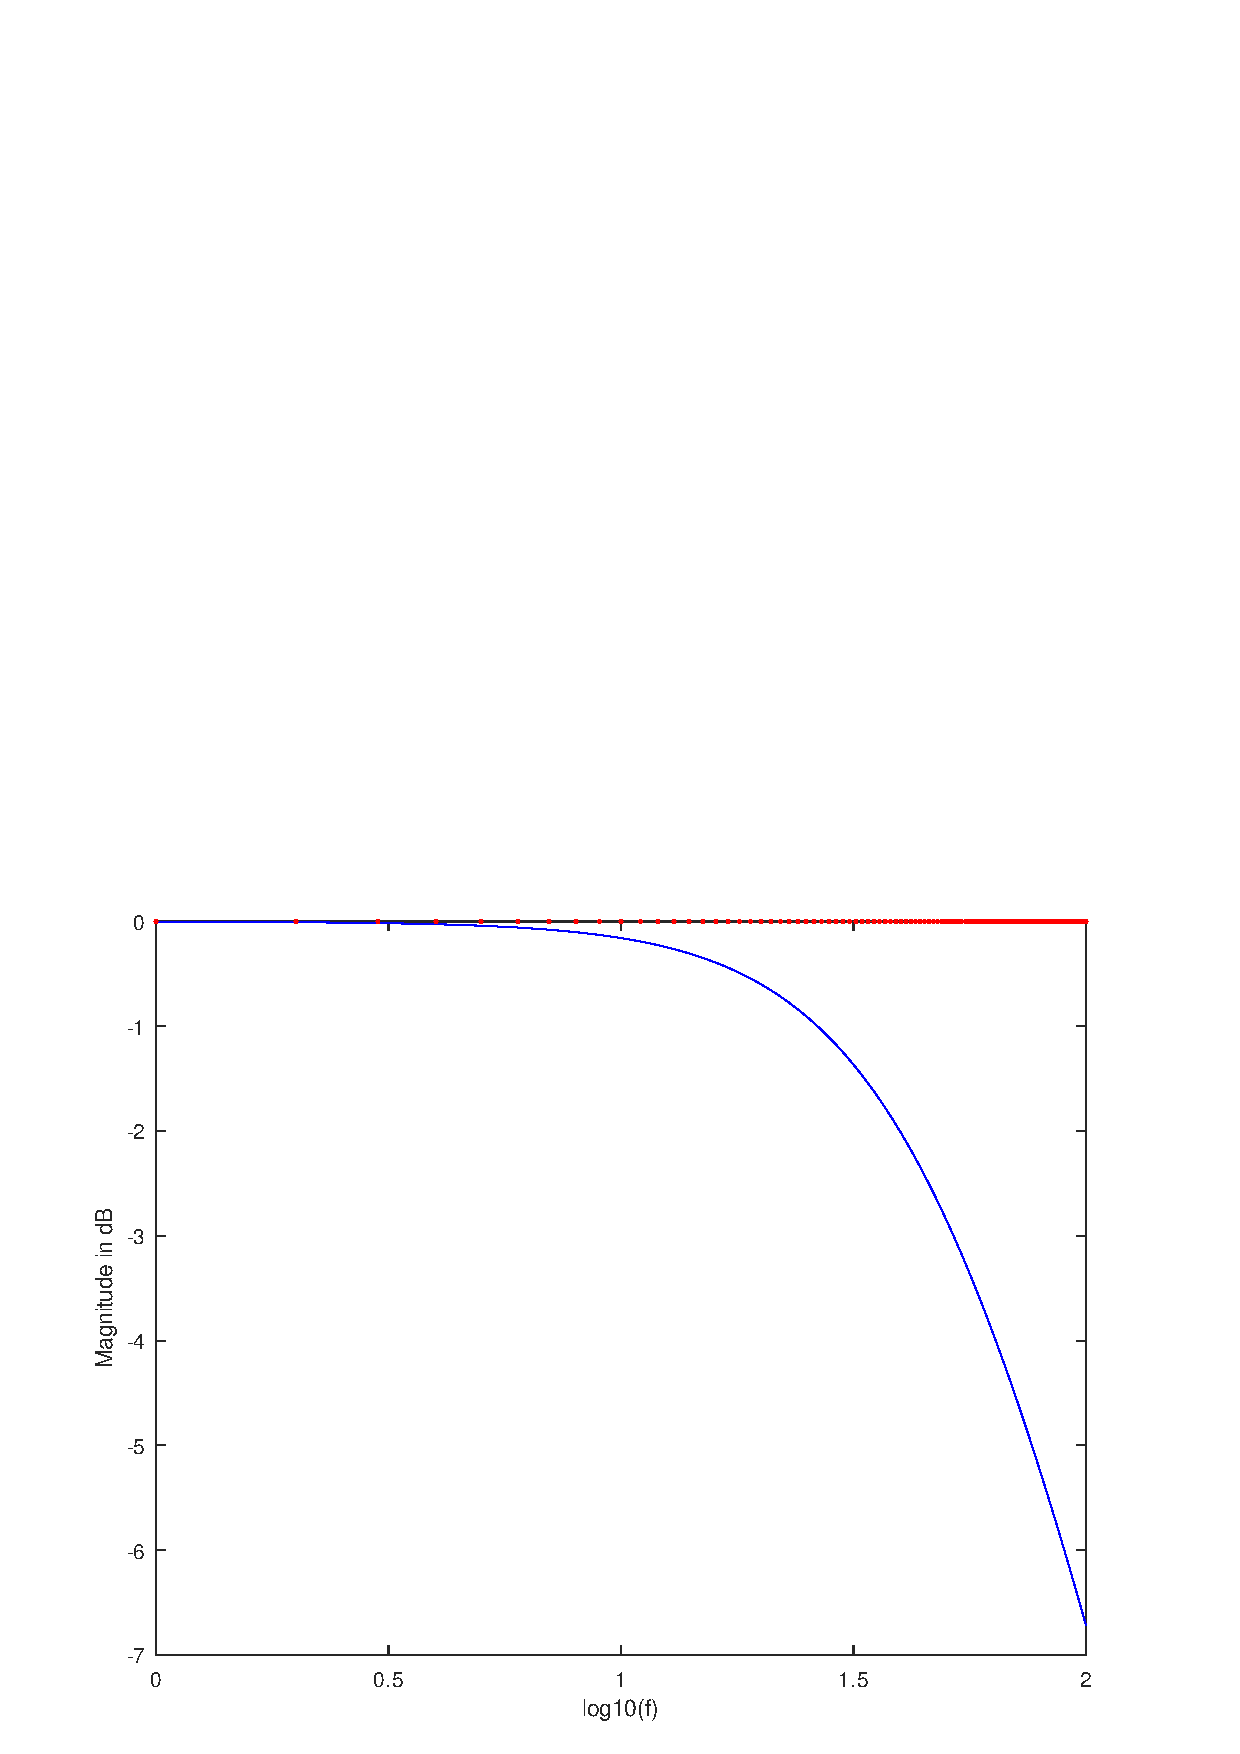
\includegraphics[width=0.7\linewidth]{magnitude.pdf}
\caption{...}
\label{fig:magnitude}
\end{figure}

\begin{figure}[h] \centering
\includegraphics[width=0.7\linewidth]{phase.pdf}
\caption{...}
\label{fig:phase}
\end{figure}
